\documentclass[10pt,aspectratio=169]{beamer}

\usetheme[progressbar=foot]{metropolis}
\AtBeginSection{}

\usepackage{appendixnumberbeamer}
\usepackage{booktabs}
\usepackage[scale=2]{ccicons}
\usepackage{tabularx}
\usepackage{tikz}
\usetikzlibrary{arrows.meta,positioning,shapes.geometric,fit,calc}
\usepackage{xspace}
\newcommand{\themename}{\textbf{\textsc{metropolis}}\xspace}
\usepackage{comment}
\usepackage{caption}
\usepackage[
  backend=biber,
  style=authoryear
]{biblatex}

\setbeamertemplate{bibliography item}{}
\addbibresource{bibliography.bib}

\usepackage{graphicx}
\usepackage{siunitx}



%................................................................................
% COLORS

\definecolor{ukudlaBlue}{RGB}{41, 60, 135}
\definecolor{ukudlaLightBlue}{RGB}{212, 216, 231}
\definecolor{ukudlaRed}{RGB}{164, 28, 34}
\definecolor{ukudlaLightRed}{RGB}{236, 209, 210}
\definecolor{ukudlaGreen}{RGB}{59, 139, 71}
\definecolor{ukudlaLightGreen}{RGB}{215, 231, 218}
\definecolor{ukudlaYellow}{RGB}{239, 198, 44}
\definecolor{ukudlaLightYellow}{RGB}{251, 243, 212}
\definecolor{white}{RGB}{255, 255, 255}
\definecolor{black}{RGB}{0, 0, 0}

\setbeamercolor{palette primary}{fg=white, bg=ukudlaGreen}
\setbeamercolor{progress bar}{fg=ukudlaRed, bg=ukudlaYellow}
\setbeamercolor{title separator}{fg=ukudlaRed, bg=ukudlaYellow}
\setbeamercolor{progress bar in head/foot}{fg=ukudlaRed, bg=ukudlaYellow}
\setbeamercolor{progress bar in section page}{fg=ukudlaRed, bg=ukudlaYellow}
\setbeamercolor{background canvas}{bg=white}
\setbeamercolor{block body}{bg=ukudlaLightGreen,fg=black}



%................................................................................
% PRESENTATION INFORMATION

\title{UKUDLA Data Science Certificate}
\subtitle{Data Integration}
\author{Markus Mößler}
\institute{University of Hohenheim}



%................................................................................
% CUSTOM FOOTER

\makeatletter
\setbeamertemplate{progress bar in head/foot}{%
  \tikzset{metropolis@progressbar@foreground/.style={fill=ukudlaGreen}}%
  \tikzset{metropolis@progressbar@background/.style={fill=ukudlaLightGreen}}%

  \begin{tikzpicture}[overlay, x=\paperwidth, y=1cm]
    \fill[metropolis@progressbar@background]
      (0,0) rectangle (1,0.10);
    \fill[metropolis@progressbar@foreground]
      (0,0) rectangle
      ({\insertframenumber/\inserttotalframenumber},0.10);
    \node[anchor=south west, yshift=0.25cm, xshift=0.2cm]
      at (0,0)
      {\includegraphics[height=0.75cm]{./logos/UKUDLA_logo_03_white_bg.pdf}};
    % current section
    \ifnum\value{section}>0
      \node[
        anchor=south east,
        yshift=0.22cm,
        xshift=-0.60cm,
        fill=ukudlaLightGreen,
        rounded corners=2pt,
        inner xsep=6pt,
        inner ysep=3pt,
        font=\scriptsize\bfseries,
        text=ukudlaRed
      ] at (1,0) {
        \insertsectionhead
      };
    \fi

  \end{tikzpicture}%
}
\makeatother



%................................................................................
% CUSTOM TITLE PAGE

\makeatletter
\setbeamertemplate{title page}{
  \begin{beamercolorbox}[sep=8pt, center, wd=\paperwidth, ht=0.5\paperheight]{title page top}
    \begin{minipage}[c]{1.00\textwidth}
      \raggedleft
      \includegraphics[height=1.00cm]{./logos/ukudla_universities.pdf}
      \vspace*{0.2cm}
    \end{minipage}
    \begin{beamercolorbox}[wd=0.9\paperwidth, sep=12pt, left]{top box}
      {\usebeamerfont{title}\usebeamercolor[fg]{title}\inserttitle\par}
      \vskip0.1cm
      {\usebeamerfont{subtitle}\usebeamercolor[fg]{subtitle}\insertsubtitle\par}
    \end{beamercolorbox}
  \end{beamercolorbox}
  \begin{beamercolorbox}[sep=8pt, center, wd=\paperwidth, ht=0.5\paperheight]{title page bottom}
    \begin{beamercolorbox}[wd=0.9\paperwidth, sep=12pt, left]{bottom box}
      \hbox{%
        \hspace*{1em}
        \begin{minipage}[c]{0.40\textwidth}
          \vskip1.0cm
          {\usebeamerfont{author}\usebeamercolor[fg]{author}\insertauthor\par}
          \vskip0.1cm
          {\usebeamerfont{institute}\usebeamercolor[fg]{institute}\insertinstitute\par}
        \end{minipage}%
        \hspace*{1.5cm}
        \begin{minipage}[c]{1.00\textwidth}
          \includegraphics[height=2.0cm]{./logos/UKUDLA_logo_05.pdf}
        \end{minipage}%
      }
    \end{beamercolorbox}
    \begin{minipage}[r]{1.00\textwidth}
      \centering
      \includegraphics[width=1.00\textwidth]{./logos/ukudla_sponsors.pdf}
    \end{minipage}
  \end{beamercolorbox}
}
\makeatother

\setbeamercolor{title page top}{bg=white}
\setbeamercolor{top box}{bg=ukudlaGreen}
\setbeamercolor{title page bottom}{bg=white}
\setbeamercolor{bottom box}{bg=ukudlaLightGreen}
\setbeamercolor{title}{fg=white}
\setbeamercolor{subtitle}{fg=white}
\setbeamercolor{author}{fg=black}
\setbeamercolor{institute}{fg=black}
\setbeamercolor{date}{fg=black}



%................................................................................
% DOCUMENT

\begin{document}

\maketitle

%--------------------------------------------------
{
\setbeamertemplate{frame numbering}[none]

\begin{frame}[noframenumbering]{Table of contents}

  \small
  \setbeamertemplate{section in toc}[sections numbered]
  \tableofcontents[hideallsubsections]

\end{frame}
}
%--------------------------------------------------



\section{Motivation}


%--------------------------------------------------
% CONTENT SLIDE 1/10
\begin{frame}{A managed dataset may not answer the question}

\small
\centering

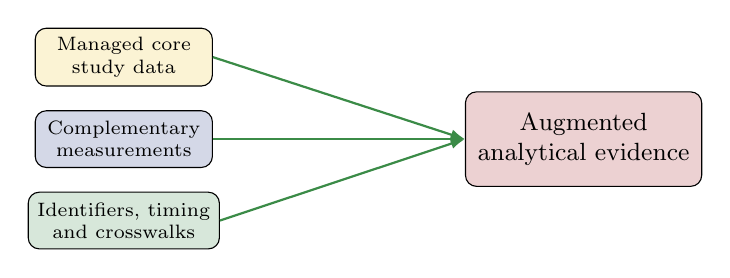
\begin{tikzpicture}[
  source/.style={
    draw,
    rounded corners,
    minimum width=2.25cm,
    minimum height=0.72cm,
    align=center,
    font=\scriptsize
  },
  result/.style={
    draw,
    rounded corners,
    minimum width=3.0cm,
    minimum height=1.2cm,
    align=center,
    font=\small
  },
  arrow/.style={-{Latex[length=1.8mm]},thick,ukudlaGreen}
]
  \node[source,fill=ukudlaLightYellow] (core) {Managed core\\study data};
  \node[source,fill=ukudlaLightBlue,below=0.30cm of core] (additional) {Complementary\\measurements};
  \node[source,fill=ukudlaLightGreen,below=0.30cm of additional] (boundaries) {Identifiers, timing\\and crosswalks};
  \node[result,fill=ukudlaLightRed,right=3.2cm of additional] (integrated) {Augmented\\analytical evidence};
  \draw[arrow] (core.east) -- (integrated.west);
  \draw[arrow] (additional.east) -- (integrated.west);
  \draw[arrow] (boundaries.east) -- (integrated.west);
\end{tikzpicture}

\vspace{0.45cm}

\raggedright

One managed source rarely contains every outcome, exposure, treatment,
covariate or context required by a study. Additional measurements or datasets
can add evidence---if their observations can be aligned responsibly.

\vspace{0.25cm}

\begin{beamercolorbox}[rounded=true,sep=8pt]{block body}
Data integration combines information from different sources into a coherent unit of analysis while preserving meaning and lineage.
\end{beamercolorbox}

\end{frame}
%--------------------------------------------------


%--------------------------------------------------
% CONTENT SLIDE 2/10
\begin{frame}{Data integration extends data management}

\small

\begin{columns}[T]

\column{0.31\textwidth}

\textbf{Manage each source}

Describe, validate and preserve both the existing and additional data.

\column{0.31\textwidth}

\textbf{Integrate deliberately}

Align identifiers, grains, periods, spaces, units and classifications.

\column{0.31\textwidth}

\textbf{Manage the result}

Audit the join and document the new artifact, assumptions and lineage.

\end{columns}

\vspace{0.55cm}

\begin{beamercolorbox}[rounded=true,sep=8pt]{block body}
This session moves from \textbf{motivation}, through the essential
\textbf{concepts}, to an auditable \textbf{application} across compatible sources.
\end{beamercolorbox}

\vspace{0.25cm}

\centering
\textcolor{ukudlaRed}{Data acquisition supports this process; integration is the teaching focus.}

\end{frame}
%--------------------------------------------------



\section{Concepts}


%--------------------------------------------------
% CONTENT SLIDE 3/10
\begin{frame}{Sources bring different representations}

\small

\begin{columns}[T]

\column{0.48\textwidth}

\textbf{Core study data}

\begin{itemize}
  \item laboratory samples or assay results;
  \item experimental plots and treatments;
  \item observational units and visits; or
  \item entities and periods from secondary data.
\end{itemize}

\column{0.48\textwidth}

\textbf{Complementary data}

\begin{itemize}
  \item instrument, sensor or laboratory measurements;
  \item management, survey or administrative records;
  \item weather, soil or remote-sensing products; and
  \item different grains may require aggregation.
\end{itemize}

\end{columns}

\vspace{0.35cm}

\begin{beamercolorbox}[rounded=true,sep=8pt]{block body}
Different representations must be made compatible without hiding how their meaning, space and time differ.
\end{beamercolorbox}

\end{frame}
%--------------------------------------------------


%--------------------------------------------------
% CONTENT SLIDE 4/10
\begin{frame}{A data need initiates integration}

\scriptsize
\centering

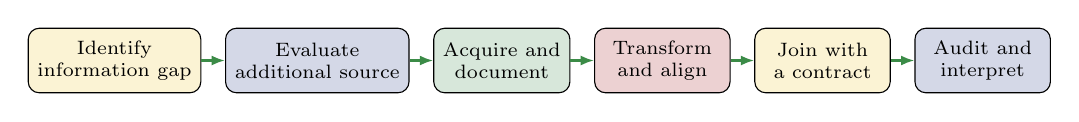
\begin{tikzpicture}[
  workflowstep/.style={
    draw,
    rounded corners,
    minimum width=1.72cm,
    minimum height=0.82cm,
    align=center,
    font=\scriptsize
  },
  arrow/.style={-{Latex[length=1.7mm]},thick,ukudlaGreen}
]
  \node[workflowstep,fill=ukudlaLightYellow] (need) {Identify\\information gap};
  \node[workflowstep,fill=ukudlaLightBlue,right=0.30cm of need] (source) {Evaluate\\additional source};
  \node[workflowstep,fill=ukudlaLightGreen,right=0.30cm of source] (record) {Acquire and\\document};
  \node[workflowstep,fill=ukudlaLightRed,right=0.30cm of record] (retrieve) {Transform\\and align};
  \node[workflowstep,fill=ukudlaLightYellow,right=0.30cm of retrieve] (preserve) {Join with\\a contract};
  \node[workflowstep,fill=ukudlaLightBlue,right=0.30cm of preserve] (validate) {Audit and\\interpret};
  \draw[arrow] (need) -- (source);
  \draw[arrow] (source) -- (record);
  \draw[arrow] (record) -- (retrieve);
  \draw[arrow] (retrieve) -- (preserve);
  \draw[arrow] (preserve) -- (validate);
\end{tikzpicture}

\vspace{0.50cm}

\small
\raggedright

The research question determines what information is missing, which source is
appropriate, and what the integrated observation should represent.

\vspace{0.20cm}

\textcolor{ukudlaRed}{Do not acquire an additional dataset before defining why and how it will be integrated.}

\end{frame}
%--------------------------------------------------


%--------------------------------------------------
% CONTENT SLIDE 5/10
\begin{frame}{Compatibility has several dimensions}

\small

\begin{columns}[T]

\column{0.47\textwidth}

\textbf{Structural compatibility}

\begin{itemize}
  \item identifiers and candidate keys;
  \item dataset grain and relationships;
  \item variable types and units;
  \item missing-value conventions; and
  \item classifications and code lists.
\end{itemize}

\column{0.47\textwidth}

\textbf{Scientific compatibility}

\begin{itemize}
  \item population and geographic support;
  \item observation and reporting periods;
  \item measurement definitions;
  \item aggregation assumptions; and
  \item fitness for the intended question.
\end{itemize}

\end{columns}

\vspace{0.35cm}

\begin{beamercolorbox}[rounded=true,sep=8pt]{block body}
A technically successful join does not prove that the combined variables refer to comparable evidence.
\end{beamercolorbox}

\end{frame}
%--------------------------------------------------



%--------------------------------------------------
% CONTENT SLIDE 6/10
\begin{frame}{State the grain before joining}

\small

\centering

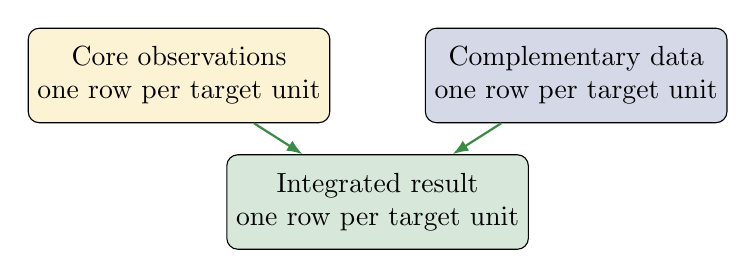
\begin{tikzpicture}[
  table/.style={
    draw,
    rounded corners,
    minimum width=3.25cm,
    minimum height=1.20cm,
    align=center
  },
  arrow/.style={-{Latex[length=2.0mm]},thick,ukudlaGreen}
]
  \node[table,fill=ukudlaLightYellow] (core)
    {Core observations\\one row per target unit};
  \node[table,fill=ukudlaLightBlue,right=1.2cm of core] (additional)
    {Complementary data\\one row per target unit};
  \node[table,fill=ukudlaLightGreen,below=1.0cm of $(core)!0.5!(additional)$] (result)
    {Integrated result\\one row per target unit};
  \draw[arrow] (core) -- (result);
  \draw[arrow] (additional) -- (result);
\end{tikzpicture}

\vspace{0.35cm}

\raggedright

\begin{itemize}
  \item A one-to-one join should preserve the expected key and row count.
  \item A one-to-many relationship can legitimately multiply rows.
  \item An unexpected many-to-many relationship often indicates an incomplete key.
  \item The join function cannot decide whether the scientific relationship is valid.
\end{itemize}

\end{frame}
%--------------------------------------------------


\section{Application}


%--------------------------------------------------
% CONTENT SLIDE 7/10
\begin{frame}{Stable identifiers and crosswalks connect sources}

\small

\begin{columns}[T]

\column{0.43\textwidth}

\textbf{Names are fragile}

\begin{itemize}
  \item spelling and punctuation differ;
  \item abbreviations differ;
  \item names and boundaries change; and
  \item the same name can identify different entities.
\end{itemize}

\column{0.53\textwidth}

\begin{tabularx}{\textwidth}{XX}
\toprule
\textbf{Source label} & \textbf{Stable ID} \\
\midrule
Plot 1 & SITE-A-P001 \\
Sample 17 & LAB-2026-0017 \\
Farm North & FARM-0042 \\
\bottomrule
\end{tabularx}

\vspace{0.35cm}

A crosswalk is a documented dataset, not an invisible correction embedded in code.

\end{columns}

\vspace{0.30cm}

\begin{beamercolorbox}[rounded=true,sep=8pt]{block body}
Check unmatched keys, duplicated keys, new missing values and row multiplication after every join.
\end{beamercolorbox}

\end{frame}
%--------------------------------------------------


%--------------------------------------------------
% CONTENT SLIDE 8/10
\begin{frame}{Integration requires alignment, not only a join}

\scriptsize

\begin{tabularx}{\textwidth}{lXX}
\toprule
\textbf{Dimension} & \textbf{Possible mismatch} & \textbf{Decision to document} \\
\midrule
Identifiers & Sample, plot, farm and provider codes & Crosswalk and valid period \\
Time & Assay, visit, season or reporting period & Alignment and period definition \\
Space & Plot, site, region, point or raster cell & Boundary, CRS, extent and summary rule \\
Units & Mass, area, concentration, rate or index & Conversion and dimensional consistency \\
Schema & Names, types, categories and flags & Mapping and retained information \\
\bottomrule
\end{tabularx}

\vspace{0.45cm}

\small

\begin{beamercolorbox}[rounded=true,sep=8pt]{block body}
Aggregating replicates, visits, sensor readings or gridded values is an analytical choice, not a neutral format conversion.
\end{beamercolorbox}

\end{frame}
%--------------------------------------------------


%--------------------------------------------------
% CONTENT SLIDE 9/10
\begin{frame}{Validate the result and preserve lineage}

\small

\begin{columns}[T]

\column{0.47\textwidth}

\textbf{Join audit}

\begin{itemize}
  \item expected and actual row counts;
  \item matched and unmatched keys;
  \item duplicated or multiplied records;
  \item missingness introduced; and
  \item resulting grain and coverage.
\end{itemize}

\column{0.47\textwidth}

\textbf{Lineage record}

\begin{itemize}
  \item source of every retained variable;
  \item crosswalks and conversion rules;
  \item temporal or spatial aggregation;
  \item script and input versions; and
  \item known losses and limitations.
\end{itemize}

\end{columns}

\vspace{0.35cm}

\begin{beamercolorbox}[rounded=true,sep=8pt]{block body}
A critical failed expectation should stop the pipeline visibly rather than produce a plausible-looking result silently.
\end{beamercolorbox}

\end{frame}
%--------------------------------------------------



%--------------------------------------------------
\section{Key Message}
% CONTENT SLIDE 10/10

\begin{frame}{Key message: integration requires explicit alignment}

\small

\centering

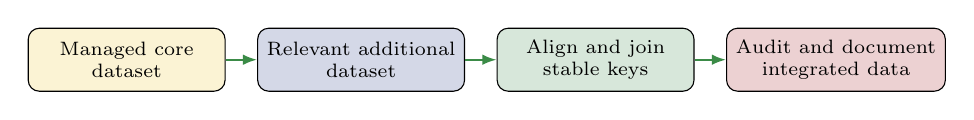
\begin{tikzpicture}[
  artifact/.style={
    draw,
    rounded corners,
    minimum width=2.50cm,
    minimum height=0.80cm,
    align=center,
    font=\scriptsize
  },
  arrow/.style={-{Latex[length=1.8mm]},thick,ukudlaGreen}
]
  \node[artifact,fill=ukudlaLightYellow] (fao) {Managed core\\dataset};
  \node[artifact,fill=ukudlaLightBlue,right=0.40cm of fao] (other) {Relevant additional\\dataset};
  \node[artifact,fill=ukudlaLightGreen,right=0.40cm of other] (join) {Align and join\\stable keys};
  \node[artifact,fill=ukudlaLightRed,right=0.40cm of join] (audit) {Audit and document\\integrated data};
  \draw[arrow] (fao) -- (other);
  \draw[arrow] (other) -- (join);
  \draw[arrow] (join) -- (audit);
\end{tikzpicture}

\vspace{0.45cm}

\raggedright

\begin{enumerate}
  \item Identify the additional information required by the question.
  \item Reconcile grain, identifiers, time, space, definitions and units.
  \item Map source labels to stable analytical identifiers.
  \item Join on tested keys under an explicit integration contract.
  \item Save the derived table, audit, dictionary and lineage record.
\end{enumerate}

\vspace{0.15cm}

\centering
\textcolor{ukudlaRed}{A successful join is not sufficient: integrated data inherit every source and alignment limitation.}

\end{frame}
%--------------------------------------------------


%--------------------------------------------------
\begin{frame}[plain,noframenumbering]{Supported by}

  South African government and the National Research Foundation

  \begin{flushleft}
    \includegraphics[trim=0cm 0cm 0cm 0cm, clip, width=0.50\textwidth]{./logos/ukudla_south_african_sponsors.pdf}
  \end{flushleft}

  German government and the German Academic Exchange Service

  \begin{flushleft}
    \includegraphics[trim=0cm 0cm 0cm 0cm, clip, width=1.00\textwidth]{./logos/ukudla_german_sponsors.pdf}
  \end{flushleft}

\end{frame}
%--------------------------------------------------

\end{document}
